\documentclass[10pt]{beamer}
\geometry{paperwidth=140mm,paperheight=110mm}
\usetheme{boxes}
\usepackage{amsmath}
\useoutertheme[subsection=false]{miniframes}
\usepackage{etoolbox}
\usepackage[english]{babel}
\usepackage{float}
\usepackage{graphicx}%for figure
\usepackage{caption}
\captionsetup{skip=0pt,belowskip=0pt}
\usepackage{algorithm}
\usepackage{algorithmicx}
\usepackage[noend]{algpseudocode}
\usepackage{multirow}
\usepackage{rotfloat}
\usepackage{lmodern}
\usepackage[export]{adjustbox}
\usepackage{subfig}

\makeatletter
\patchcmd{\slideentry}{\advance\beamer@xpos by1\relax}{}{}{}
\def\beamer@subsectionentry#1#2#3#4#5{\advance\beamer@xpos by1\relax}%
\makeatother

\setbeamercolor{footline}{fg=blue}
\addtobeamertemplate{navigation symbols}{}{%
    \usebeamerfont{footline}%
    \usebeamercolor[fg]{footline}%
    \hspace{1em}%
    \insertframenumber/\inserttotalframenumber
}

\graphicspath{{figures/}}

\begin{document}
%%%% title page
\begin{frame}
\title{Model estimation and dynamic prediction for subject-specific event probability in joint modeling using longitudinal quantile regression}


% \author{Ming Yang, Sheng Luo, Stacia M. DeSantis}
\author{Ming Yang, Sheng Luo, Stacia DeSantis}
\institute{Department of Biostatistics\\The University of Texas School of Public Health}
\date{@JSM2016\\August 2}
\maketitle
\end{frame}

%%% table of contents
\begin{frame}
\frametitle{Outline}
\tableofcontents
\end{frame}



%%%%%%%%%%%%%%%%%==BACKGROUNDS==%%%%%%%%%%%%%%%%%%%
\section{Introduction} %%%%%%%

\subsection{A motivating data}
\frame{\frametitle{A motivating data}
\begin{itemize}
\item  A prospective observational study designed to detect early neurobiological predictors of Huntington's Disease (PREDICT-HD; ClinicalTrials.gov number NCT00051324)
\item Data: 1078 participants, median follow-up time: 61 months, 40 longitudinal biomarkers, time to HD onset and other demographic information
\item Primary focus: to measure the association between longitudinal biomarkers and the risk of HD onset
% , the clinical question lends itself to a joint modelsing approach
\item More extreme values in longitudinal biomaker(s) are associated with higher risk of HD onset
\item Many of the longitudinal biomakers are skewed
\end{itemize}
}


\frame{\frametitle{PREDICT-HD study: skewed longitudinal biomarker}
Total Motor Score (TMS), a commonly used rating criteria of body motion abilities based on the Unified Huntington Disease Rating Scale (UHDRS).
\begin{center}
\begin{figure}
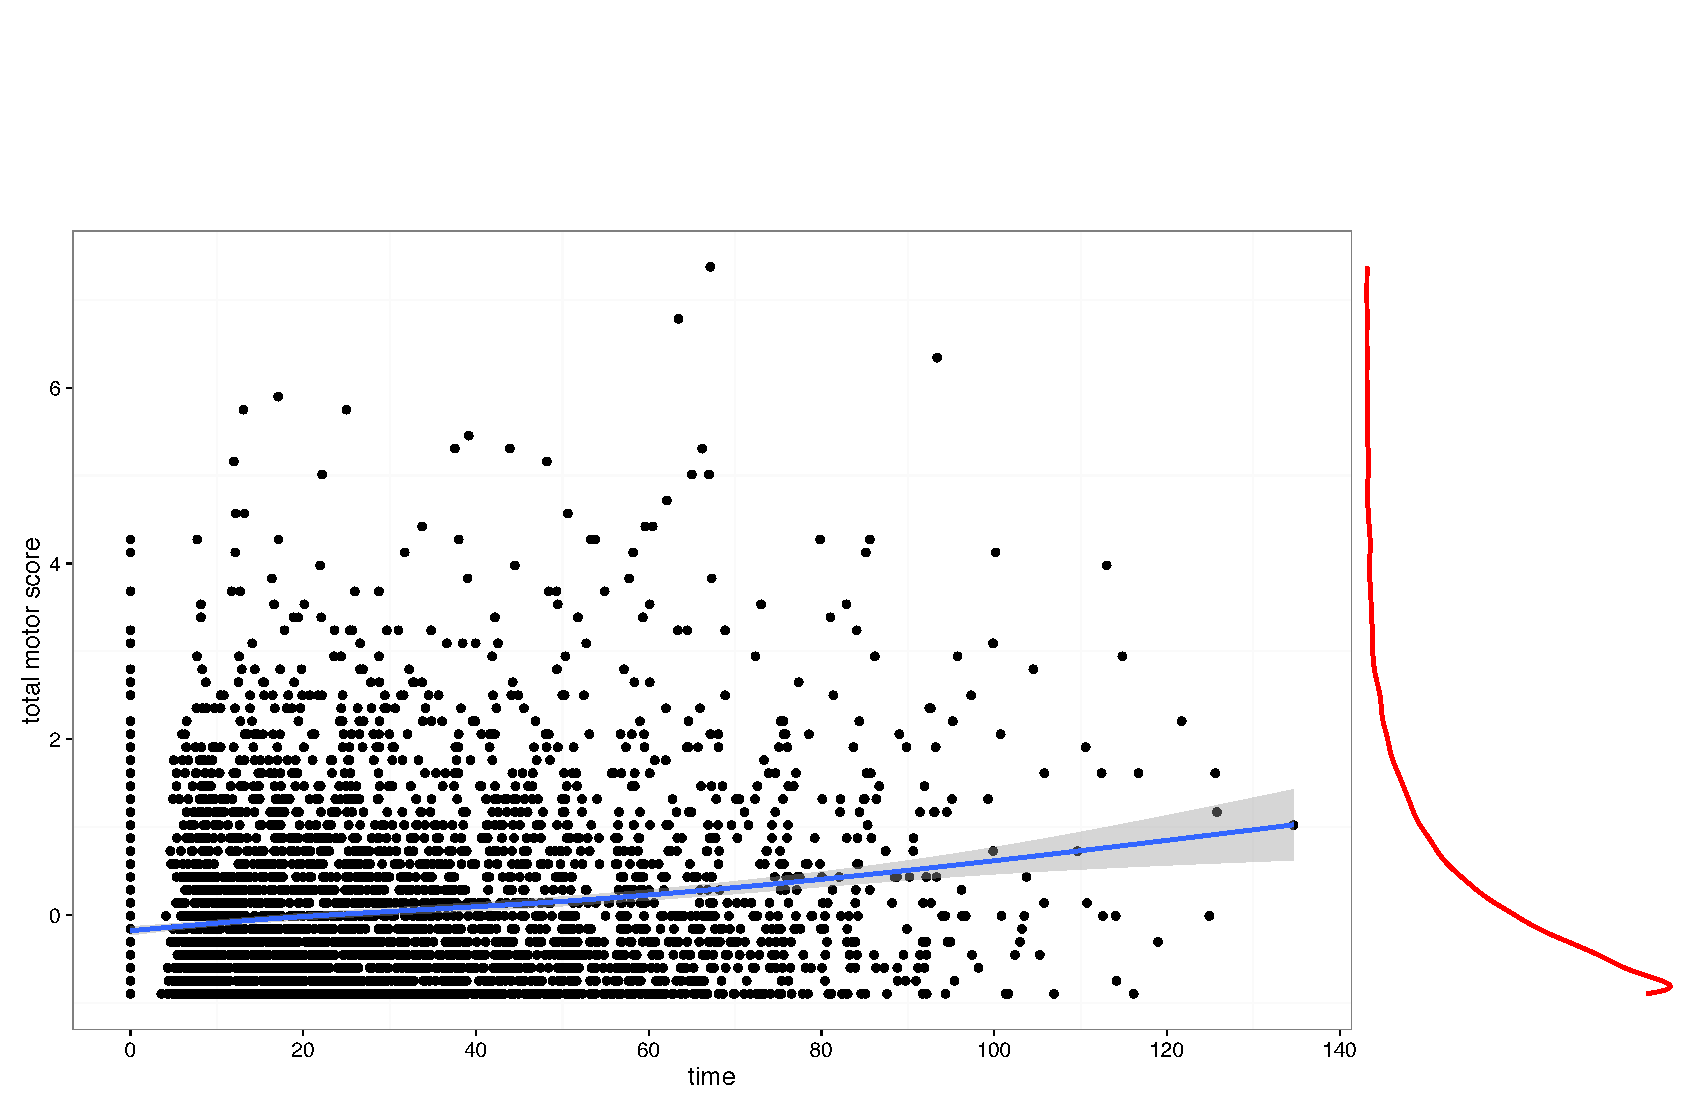
\includegraphics[scale=0.35]{neurotot_densities_loess.eps}\vspace{-2pt}
\caption{Scatter plot with LOESS curve (blue)) and kernel density plot (red) for total motor score from the study population (time unit: month; lower total motor score is better).}
\end{figure}
\end{center}
}


\subsection{Joint models for longitudinal and survival data} %
\frame{\frametitle{Joint models for longitudinal and survival data}
% \vspace{-2em}
% \begin{center}
% \begin{figure}
% 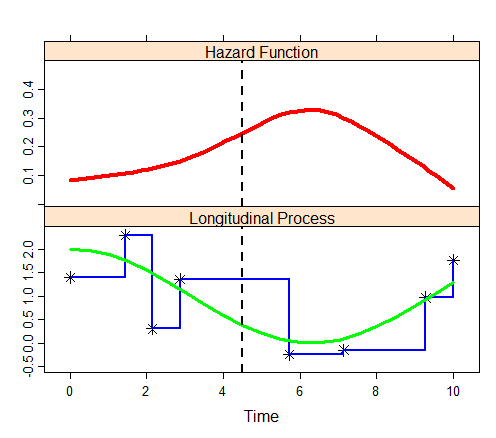
\includegraphics[scale=0.3]{JMidea.png}
% \caption{Rizopoulos, 2014 (online)}
% \end{figure}
% \end{center}
% \vspace{-1.8em}

\begin{itemize}

\item Traditional joint models (JM)
\small{
\begin{equation*}\label{eqn:joint1}
\left\{
\begin{array}{l}
Y_{i}(t) =m_{i}(t)+\varepsilon_{i}(t)= {\boldsymbol X}_{i}^{\top}(t)\boldsymbol{\beta} + {\boldsymbol Z}_{i}^{\top}(t){\boldsymbol u}_i + \varepsilon_{i}(t), \varepsilon_{i}(t)\overset{iid}{\sim} N(0, \sigma^2)\\
h(t|\mathcal{M}_{i}(t), {\boldsymbol W}_i;  \boldsymbol{\gamma}, \alpha) = h_0(t)\exp({\boldsymbol W}_i^{\top}\boldsymbol{\gamma} + \alpha m_{i}(t))
\end{array}
\right.
\end{equation*}
}

\item Linear mixed model (LMM) for the longitudinal process
\item Proportional hazards model (PHM) for the survival process
\item Longitudinal outcome is treated as a time-dependent covariate in the survival submodel
\end{itemize}

}


\frame{\frametitle{Limitations of traditional JM}

\begin{itemize}
\item LMM is sensitive to outliers and deviation of normality
\item The normality of the error term cannot be satisfied in many cases (even after applying various outcome transformations)
\item LMM models only the conditional mean of the outcome -- not very meaningful from clinical perspective in some cases
\end{itemize}
}



\subsection{Research questions} %%%%%%%
\frame{\frametitle{Research questions}
\begin{enumerate}
\item How to deal with the non-normality in the data?
\item How to study the covariates effect on the higher/lower tail of the biomarkers?
\item How to make predictions of HD-free probability in the future? Dynamically?
\end{enumerate}
}


%%%%%%%%%%%%%%%%%==METHODS==%%%%%%%%%%%%%%%%%%%%%%%%
\section{Statistical methods} %%%%%%%

\frame{\frametitle{Statistical methods}
\begin{itemize}
\item JM using longitudinal quantile regression
\item Subject-specific dynamic predictions
\end{itemize}

}



\subsection{Review of quantile regression} %%%%%%%
\frame{\frametitle{Quantile Regression (QR)}

\begin{itemize}

\item QR models%s a specific quantile of the outcome as a linear function of the covariates:
\begin{equation}\label{eqn:lqr}
Q_{Y|{\boldsymbol X}}(\tau)={\boldsymbol X}^{\top}\boldsymbol{\beta}_{\tau},
\end{equation}
where the $\tau$th quantile of a random variable $Y$, $\tau\in[0,1]$, is defined as
\begin{equation*}\label{eqn:quantile}
Q_{Y}(\tau)=F_{Y}^{-1}(\tau)=\inf\left\{ y:Pr(Y\le y)\geq\tau\right\}.
\end{equation*}

\item Regression parameters are estimated as:
\begin{equation}\label{eqn:loss_fun}
\hat{\boldsymbol{\beta}}_{\tau}=\underset{\boldsymbol{\beta}\in \mathbb{R}^{p}}{\mbox{arg min}}\sum_{i=1}^{n}\left[\rho_{\tau}(Y_{i}-{\boldsymbol X}_i^{\top}\boldsymbol{\beta}_{\tau})\right],
\end{equation}
where $\rho_{\tau}(Y)=Y(\tau-{I}{(Y<0)}).$
%\item There is no direct solution for Equation (\ref{eqn:loss_fun}), and linear programming method can be used to solve it.
\end{itemize}

}


\frame{\frametitle{Parameter estimation from QR vs. mean regression}
\begin{center}
\begin{figure}
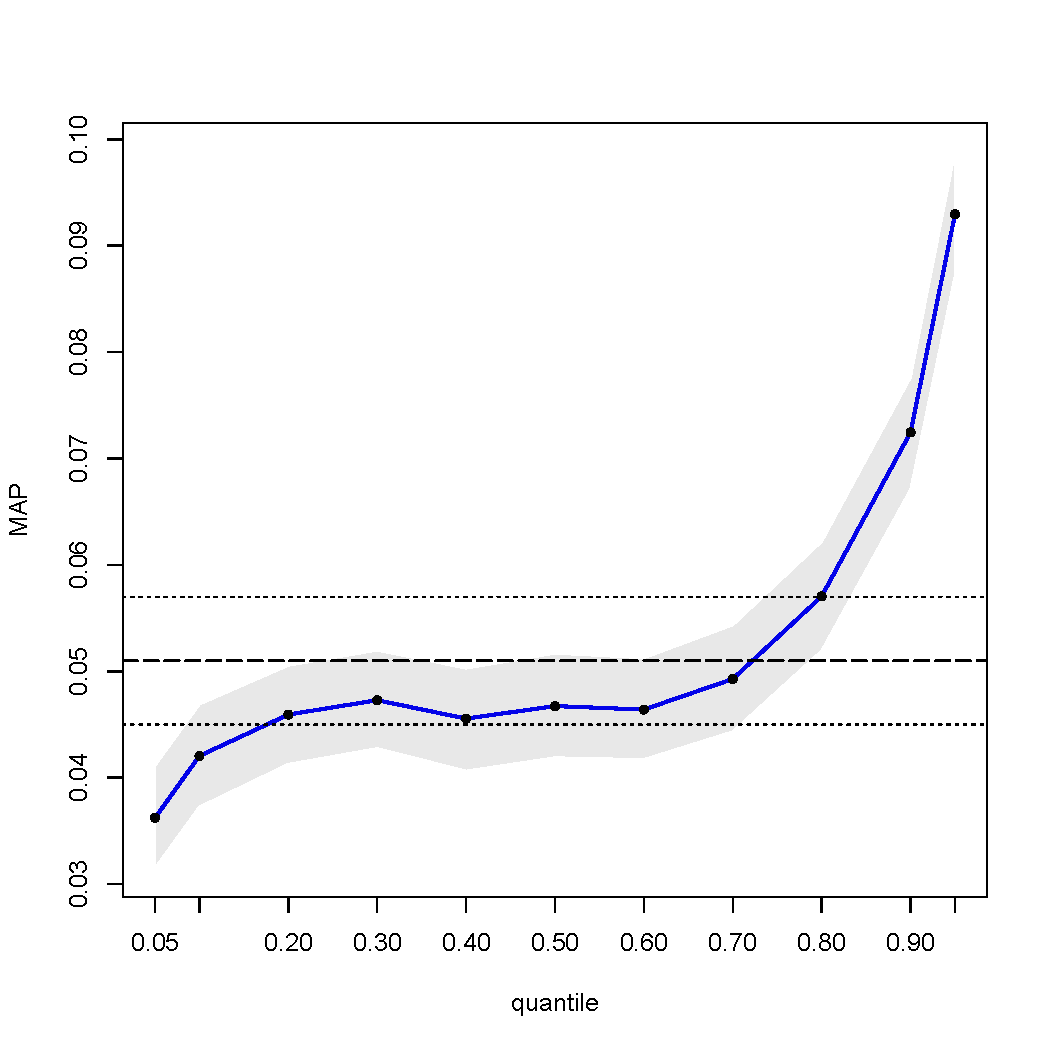
\includegraphics[scale=0.45]{MAP.pdf}
\caption{Quantile effect v.s. mean effect}
\end{figure}
\end{center}


}


\subsection{JM using longitudinal quantile regression} %%%%%%%
\frame{\frametitle{Longitudinal quantile regression}

\begin{itemize}
\item The linear quantile mixed model (LQMM):
\[
\left\{
\begin{array}{l}
Y_{i}(t)={\boldsymbol X}_{i}^{\top}(t) \boldsymbol{\beta}_{\tau}+ {\boldsymbol Z}_{i}^{\top}(t)\boldsymbol{u}_i + \varepsilon_i(t),\ i=1, \cdots, N;\ t=1,\cdots, n_i,\\
Q_{Y_{i}(t)|{\boldsymbol X}_{i}, {\boldsymbol Z}_{i}, \boldsymbol{u}_i}(\tau) = {\boldsymbol X}_{i}^{\top}(t) \boldsymbol{\beta}_{\tau}+ {\boldsymbol Z}_{i}^{\top}(t)\boldsymbol{u}_i
\end{array}
\right.
\]\label{eqn:lqmm}

\item Assume asymmetric Laplace distribution (ALD) of the random error, i.e. $\varepsilon_{i}(t)\overset{iid}\sim $ ALD$(0, \sigma, \tau)$:
\begin{equation*}\label{eqn:ald}
f(\varepsilon_{i}(t)|\mu, \sigma, \tau)=\frac{\tau(1-\tau)}{\sigma}\exp\left[-\rho_{\tau}\left(\frac{\varepsilon_{i}(t)}{\sigma}\right)\right];
\end{equation*}

\item Then $Y_{i}(t)|{\boldsymbol X}_{i}, {\boldsymbol Z}_{i}, \boldsymbol{u}_i\overset{iid}\sim$ ALD(${\boldsymbol X}_{i}^{\top}(t)\boldsymbol{\beta}+{\boldsymbol Z}_{i}^{\top}(t)\boldsymbol{u}_i, \sigma, \tau$):

\begin{equation*}\label{eqn:ald_lqmm}
f(Y_{i}(t)|{\boldsymbol X}_{i}, {\boldsymbol Z}_{i}, \boldsymbol{u}_i;\boldsymbol{\beta},\sigma)=\frac{\tau(1-\tau)}{\sigma}\exp\left[-\rho_{\tau}\left(\frac{Y_{i}(t)-{\boldsymbol X}_{i}^{\top}(t)\boldsymbol{\beta}-{\boldsymbol Z}_{i}^{\top}(t)\boldsymbol{u}_i}{\sigma}\right)\right].
\end{equation*}

\end{itemize}
  }



\frame{\frametitle{ALD vs. LD vs. Normal}
In ALD($\mu, \sigma, \tau$), $\mu\in(-\infty, \infty)$ is the location parameter, $\sigma$ is the scale parameter and $\tau\in(0, 1)$ is the parameter that control the skewness of the distribution.

\begin{center}
\begin{figure}
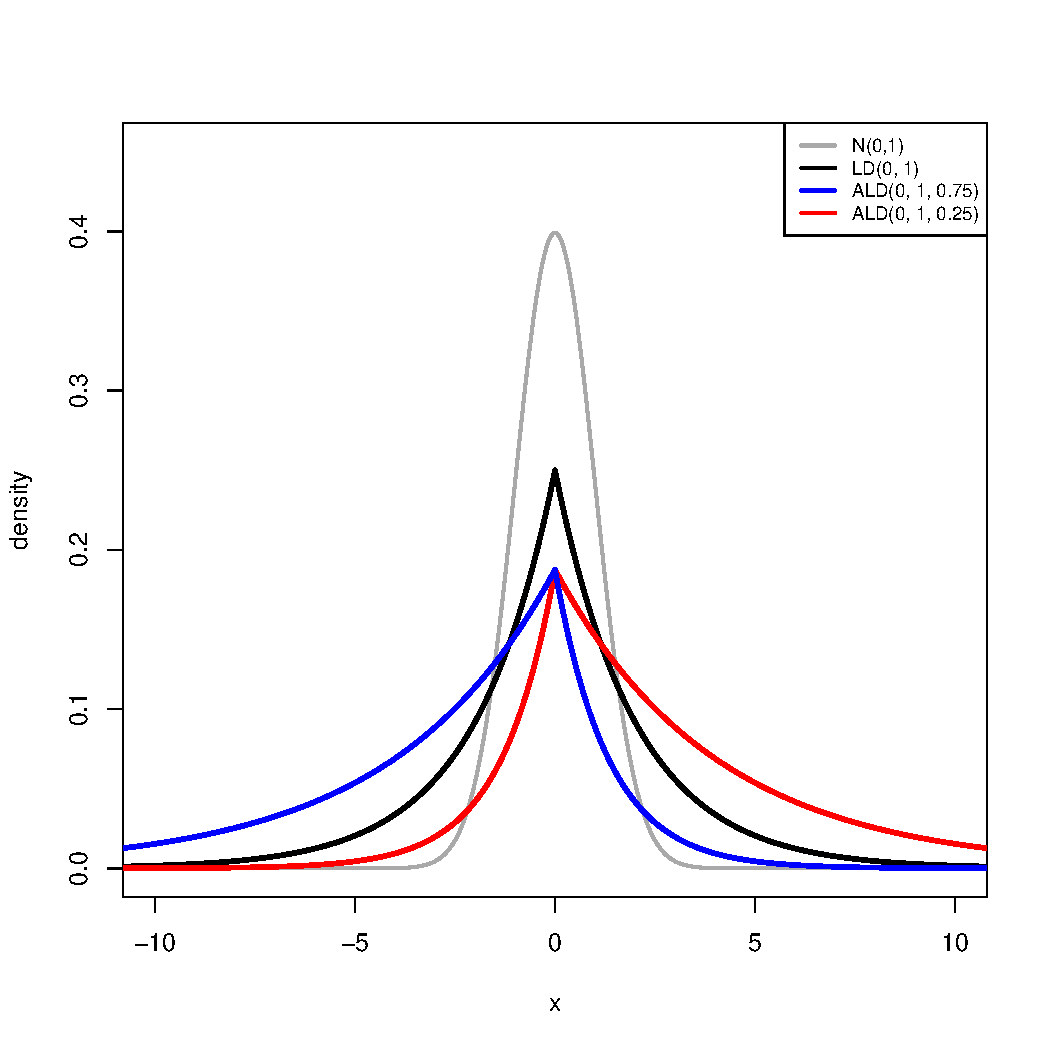
\includegraphics[scale=0.35]{ald_ld_normal.pdf}\vspace{-2pt}
\caption{Asymmetric Laplace, Laplace, and normal distributions}
\end{figure}
\end{center}
}



% \frame{\frametitle{Reparametrization of ALD}
% \begin{itemize}
% \item The location-scale mixture representation of the ALD (Kotz et al., 2001):

% \[\varepsilon_{ij}=\kappa_1e_{ij}+\kappa_2\sqrt{\sigma e_{ij}}v_{ij}.\]

% \item Then the model becomes:
% \begin{equation}\label{eqn:reformald2}
% Y_{ij}={\boldsymbol X}_{ij}^{\top}\boldsymbol{\beta}+{\boldsymbol Z}_{ij}^{\top}\boldsymbol{u}_i+\kappa_1e_{ij}+\kappa_2\sqrt{\sigma e_{ij}}v_{ij}.
% \end{equation}

% where
% \[\kappa_1=\frac{1-2\tau}{\tau(1-\tau)}, \kappa_2^2=\frac{2}{\tau(1-\tau)},\]
% and \[v_{ij}\sim N(0,1), e_{ij}\sim\exp(1/\sigma).\]

% \end{itemize}
%   }



\frame{\frametitle{Quantile regression joint models (QRJM)}
{\small
\begin{equation}\label{eqn:QRJM}
\left\{
\begin{array}{l}
Y_{i}(t) = m_{i}(t) + \varepsilon_{i}(t) = {\boldsymbol X}_{i}^{\top}(t)\boldsymbol{\beta}_{\tau} + {\boldsymbol Z}_{i}^{\top}(t){\boldsymbol u}_i + \varepsilon_{i}(t), \varepsilon_{i}(t)\sim ALD(0, \sigma, \tau)\\
h(T_i|\mathcal{M}_{i}(T_i), {\boldsymbol W}_i;  \boldsymbol{\gamma}_{\tau}, \alpha_{\tau}) = h_0(T_i)\exp({\boldsymbol W}_i^{\top}\boldsymbol{\gamma}_{\tau} + \alpha_{\tau}({\boldsymbol X}^{\top}_{i}(T_i)\boldsymbol{\beta}_{\tau} + {\boldsymbol Z}^{\top}_{i}(T_i){\boldsymbol u}_{i}))
\end{array}
\right.
\end{equation}
}

where:
\begin{itemize}
\item $m_i(t)$: the error-free longitudinal measure; $\mathcal{M}_{i}(T_i)=\{m_i(s): 0\le s\le T_i\}$
\item $T_i=\min(T_i^*, C_i)$: the event time for subject $i$, where $T_i^*$ is the true underlying event time and $C_i$ is the censoring time
\item $\boldsymbol{\beta}, \boldsymbol{\gamma}$: the fixed effects
\item $\boldsymbol{u}_i$: a vector of random effects for subject $i$
\item $\alpha$: the parameter governing the strength of association
\end{itemize}
}


\subsection{Dynamic prediction of event-free probabilities}%%%%%%%%%%
\frame{\frametitle{Dynamic prediction of future event-free probabilities}
\begin{itemize}



\item The predicted probability of no event until time $m$ given no event until time $t$ $(t<m)$ is given by

{\small
\begin{eqnarray}\label{eqn:surv_prob_derv}
&&\nonumber Pr(T_i^*\ge m|T_i^*>t, \mathcal{Y}_i(t), \mathcal{D}_n;\boldsymbol{\theta})\\
&=&\int\frac{{S}_i[m|\mathcal{M}_i(m, u_i, \boldsymbol{\theta});\boldsymbol{\theta}]}{{S}_i[t|\mathcal{M}_i(t, u_i, \boldsymbol{\theta});\boldsymbol{\theta}]}Pr(u_i|T_i^*>t, \mathcal{Y}_i(t);\boldsymbol{\theta})du_i,
\end{eqnarray}}

\item Notations:
\begin{itemize}
\item $p_i(m|t) = Pr(T_i^*\ge m|T_i^*>t, \mathcal{Y}_i(t), \mathcal{D}_n;\boldsymbol{\theta})$: the probability that patient $i$ is free of event up to time $m>t$, given he/she is free of event until time $t$
\item $\mathcal{Y}_i(t)=\{Y_i(s), 0\le s\le t\}$: complete history of observed longitudinal outcome for patient $i$ up to time $t$
\item $\mathcal{D}_n=\{T_i, \Delta_i, \boldsymbol{Y}_i, i=1, \cdots, n\}$: the training data
\end{itemize}
\end{itemize}
}


\frame{\frametitle{Estimation of the predicted probability}
{\small
\begin{itemize}

\item Generate Monte Carlo samples of $p_i(m|t)$: %upon collecting
\begin{itemize}
\item draw $\boldsymbol{\theta}^{(k)}\sim f(\boldsymbol{\theta}|\mathcal{D}_n)$;
\item draw $u^{(k)}_i\sim f(u_i|T_i^*>t, \mathcal{Y}_i(t), \boldsymbol{\theta}^{(k)})$;
\item compute $p_i^{(k)}(m|t)=S_i[m|\mathcal{M}_i(m, u^{(k)}_i, \boldsymbol{\theta}^{(k)});\boldsymbol{\theta}^{(k)}]S_i[t|\mathcal{M}_i(t, u^{(k)}_i, \boldsymbol{\theta}^{(k)});\boldsymbol{\theta}^{(k)}]^{-1}$
\end{itemize}

\item Approximate the true value using sample mean or median:
\begin{equation}\label{eqn:sample_mean}
\hat{p}_i(m|t)=\frac{1}{K}\sum_{k=1}^K p^{(k)}_i(m|t).
\end{equation}

\end{itemize}
}
  }



\subsection{Predictive performance} %%%%%%%
\frame{\frametitle{Statistics to assess predictive performance}
\begin{itemize}
\item Let $\hat{r}_i(t+\Delta t | t) = 1- \hat{S}_i(t+\Delta t| \mathcal{Y}_{i}(t), {\boldsymbol u}_i;\boldsymbol{\theta}), i = 1, \cdots, N.$

\item Then
\begin{equation*}\label{est_TPR}
\widehat{TPR}_{t}^{\Delta t}(p) = \frac{\sum_{i=1}^{N}\hat{r}_i(t+\Delta t|t)I(\hat{r}_i(t+\Delta t|t)\ge p)}{\sum_{i=1}^{N}\hat{r}_i(t+\Delta t|t)},
\end{equation*}
\begin{equation*}\label{est_FPR}
\widehat{FPR}_{t}^{\Delta t}(p) = \frac{\sum_{i=1}^{N}\left(1-\hat{r}_i(t+\Delta t|t)\right)I(\hat{r}_i(t+\Delta t|t)\ge p)}{\sum_{i=1}^{N}\left(1-\hat{r}_i(t+\Delta t|t)\right)}.
\end{equation*}

\item We use the following three statistics as measures of predictive performance:
\begin{equation*}\label{est_AUC}
\widehat{AUC}_t^{\Delta t} = \int \widehat{TPR}_t^{\Delta t}\left\{ (\widehat{FPR}_t^{\Delta t})^{-1}(u)\right\}du,
\end{equation*}

\begin{equation*}\label{est_AARD}
\widehat{AARD}_t^{\Delta t} = \widehat{TPR}_t^{\Delta t}(\hat{\rho}) - \widehat{FPR}_t^{\Delta t}(\hat{\rho}),
\end{equation*}

\begin{equation*}\label{est_MRD}
\widehat{MRD}_t^{\Delta t} = \int_p \widehat{TPR}_t^{\Delta t}(p)dp - \int_p \widehat{FPR}_t^{\Delta t}(p)dp,
\end{equation*}

\noindent where $\hat{\rho} = \frac{\sum_{i=1}^N \hat{r}_i(t+\Delta t| t)}{N}$ is the average risk in the study population at time $t+\Delta t$.

\end{itemize}
  }



%%%%%%%%%%%%%%%%%==SIMULATION==%%%%%%%%%%%%%%%%%%%%%%%%
\section{Simulation studies} %%%%%%%

\subsection{Model inference}
\frame{\frametitle{Simulation study 1: model inference}
\begin{itemize}
\item Simulate data from Equation (\ref{eqn:QRJM}) and consider the following three scenarios:
  \begin{enumerate}
  \item Scenario 1: choose $\tau=$ 0.25 for the ALD
  \item Scenario 2: choose $\tau=$ 0.5 for the ALD (i.e, median equals 0)
  \item Scenario 3: random error follows standard normal distribution
  \end{enumerate}

\item For each scenario, simulate 200 data sets with $N=600$ in each.
\item Among the 600 subjects, randomly select 500 as the training data used to fit the model, and use the remaining 100 subjects as the testing data to make out-of-sample predictions in Simulation 2.
\item Compare the bias, standard error (SE), mean square error (MSE), and coverage probability (CP) for QRJM and the standard JM (LMJM).
\end{itemize}
}


\frame{\frametitle{Simulation 1 results}

\begin{table}[H]
\begin{center}
\caption{Simulation study: Inference results for data generated from ALD with $\tau=0.25$ (Scenario 1).}
\adjustbox{max width=\textwidth}{
\label{tab:sim1tab1}
\begin{tabular}{lrcccccccccccccc}
\hline
& \multicolumn{4}{c}{QRJM ($\tau=0.25$, true model)} & & \multicolumn{4}{c}{QRJM ($\tau=0.5$)} & & \multicolumn{4}{c}{LMJM}\\
\hline
 & Bias & SE & MSE & CP && Bias & SE & MSE & CP && Bias & SE & MSE & CP \\
  \hline
$\alpha$ & -0.004 & 0.078 & 0.010 & 0.970 && -0.051 & 0.119 & 0.070 & 0.930 && -0.087 & 0.103 & 0.040 & 0.800  \\
  $\beta_0$ & -0.003 & 0.080 & 0.014 & 0.930 && 1.659 & 0.129 & 2.807 & 0.020 && 2.702 & 0.146 & 7.350 & 0.000 \\
  $\beta_{11}$ & 0.015 & 0.068 & 0.010 & 0.950 && 0.024 & 0.105 & 0.043 & 0.890 && 0.080 & 0.116 & 0.052 & 0.860  \\
  $\beta_{12}$ & 0.016 & 0.083 & 0.013 & 0.950 && 0.014 & 0.112 & 0.042 & 0.970 && 0.078 & 0.128 & 0.052 & 0.920  \\
  $\gamma_1$ & 0.005 & 0.055 & 0.006 & 0.940 && 0.008 & 0.057 & 0.006 & 0.960 && 0.009 & 0.058 & 0.007 & 0.960  \\
  $\gamma_2$ & 0.006 & 0.055 & 0.006 & 0.930 && 0.010 & 0.056 & 0.007 & 0.910 && 0.010 & 0.058 & 0.007 & 0.940  \\
  % $\sigma$ & 0.000 & 0.029 & 0.002 & 0.940 && -0.321 & 0.021 & 0.104 & 0.000 && - & - & - & - && - & - & - & - \\
   \hline
\end{tabular}
}
\end{center}
\end{table}

\begin{table}[H]
\centering
\caption{Inference results for data generated from $N(0, 1)$ (Scenario 3).}
\adjustbox{max width=\textwidth}{
\label{tab:sim1tab3}
\begin{tabular}{lccccccccc}
\hline
& \multicolumn{4}{c}{QRJM ($\tau=0.5$)} & & \multicolumn{4}{c}{LMJM (true model)} \\
\hline
 & Bias & SE & MSE & CP & & Bias & SE & MSE & CP \\
 \cline{2-5}  \cline{7-10}
$\alpha$ & -0.013 & 0.055 & 0.006 & 0.95 & & 0.007 & 0.055 & 0.006 & 0.95 \\
  $\beta_0$ & 0.015 & 0.037 & 0.003 & 0.95 & & 0.000 & 0.035 & 0.002 & 0.98 \\
  $\beta_{11}$ & 0.004 & 0.034 & 0.002 & 0.96 & & -0.003 & 0.033 & 0.002 & 0.95\\
  $\beta_{12}$ & 0.013 & 0.050 & 0.005 & 0.95 & & 0.006 & 0.049 & 0.005 & 0.95 \\
  $\gamma_1$ & 0.008 & 0.055 & 0.006 & 0.92 & & 0.003 & 0.054 & 0.006 & 0.90 \\
  $\gamma_2$ & 0.015 & 0.055 & 0.007 & 0.92 & & 0.010 & 0.054 & 0.006 & 0.92 \\
   \hline
\end{tabular}
}
\end{table}

}



\subsection{Dynamic prediction}
\frame{\frametitle{Simulation 2: dynamic prediction}
\begin{itemize}
\item Use the 100 subjects as testing data and make out-of-sample predictions
\item Compare the predicted values with the true simulated values (``gold standard'')
\item Use different combinations of $(t, \Delta t)$ for prediction to mimic the real-world situation
\end{itemize}
}


\frame{\frametitle{Simulation 2 results: Bland Altman plot}
\begin{figure}[H]
\centering
\subfloat[][QRJM with $\tau=0.25$ (True model)]{
    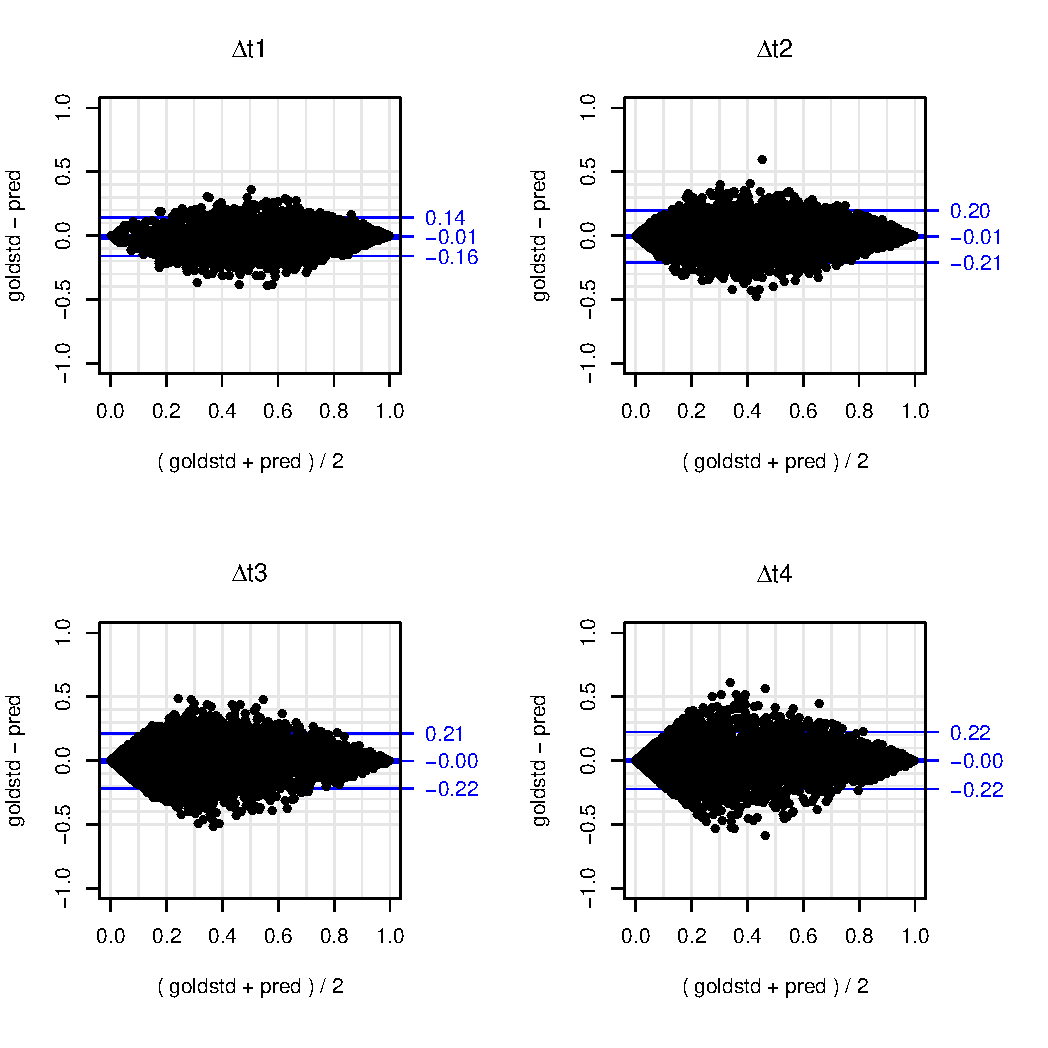
\includegraphics[width=0.45\columnwidth]{baplot_qt25data_qt25fit_jags_t1.pdf}\label{plot:sim2fig11}
}
% \centering
% \subfloat[][QRJM with $\tau=0.5$]{
%     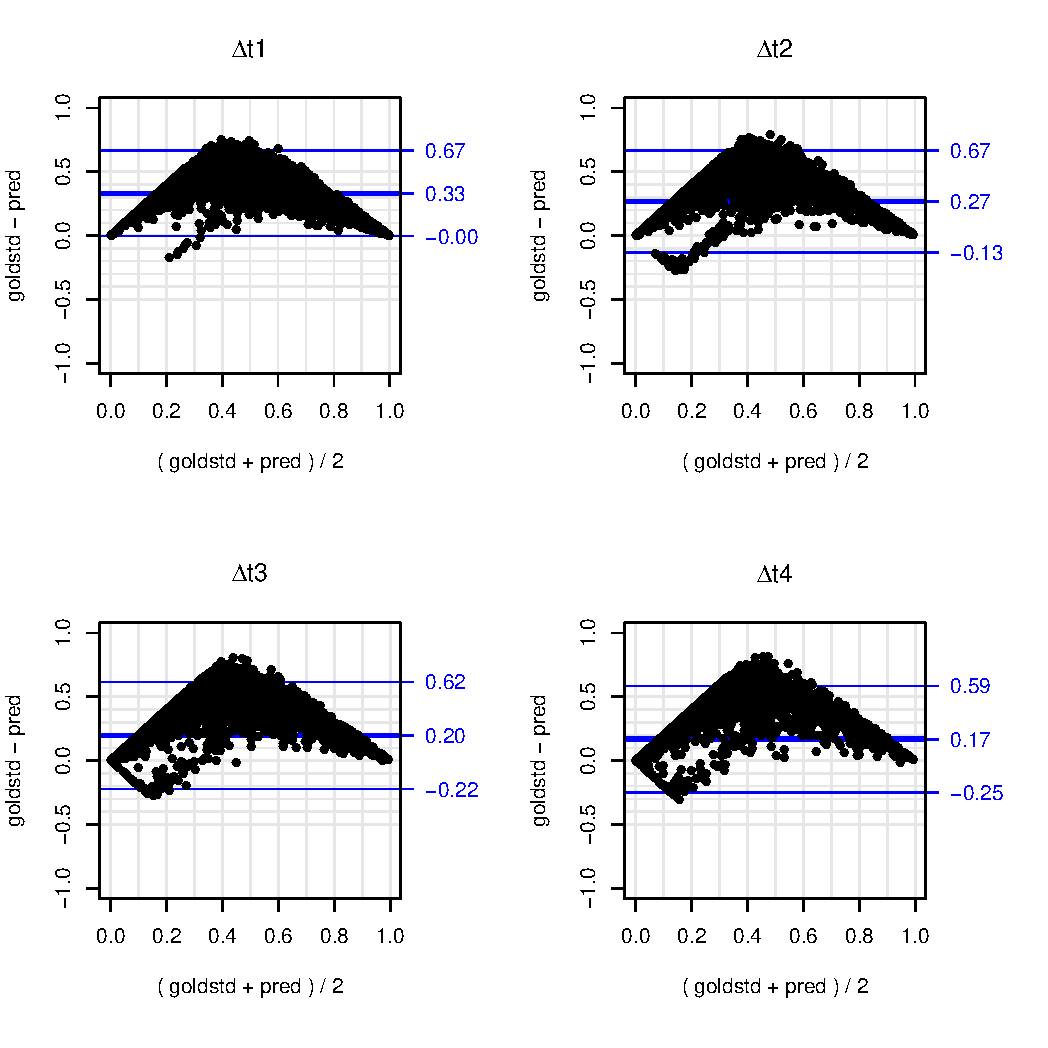
\includegraphics[width=0.4\columnwidth]{baplot_qt25data_qt50fit_jags_t1.pdf}\label{plot:sim2fig12}
% }
\subfloat[][LMJM]{
    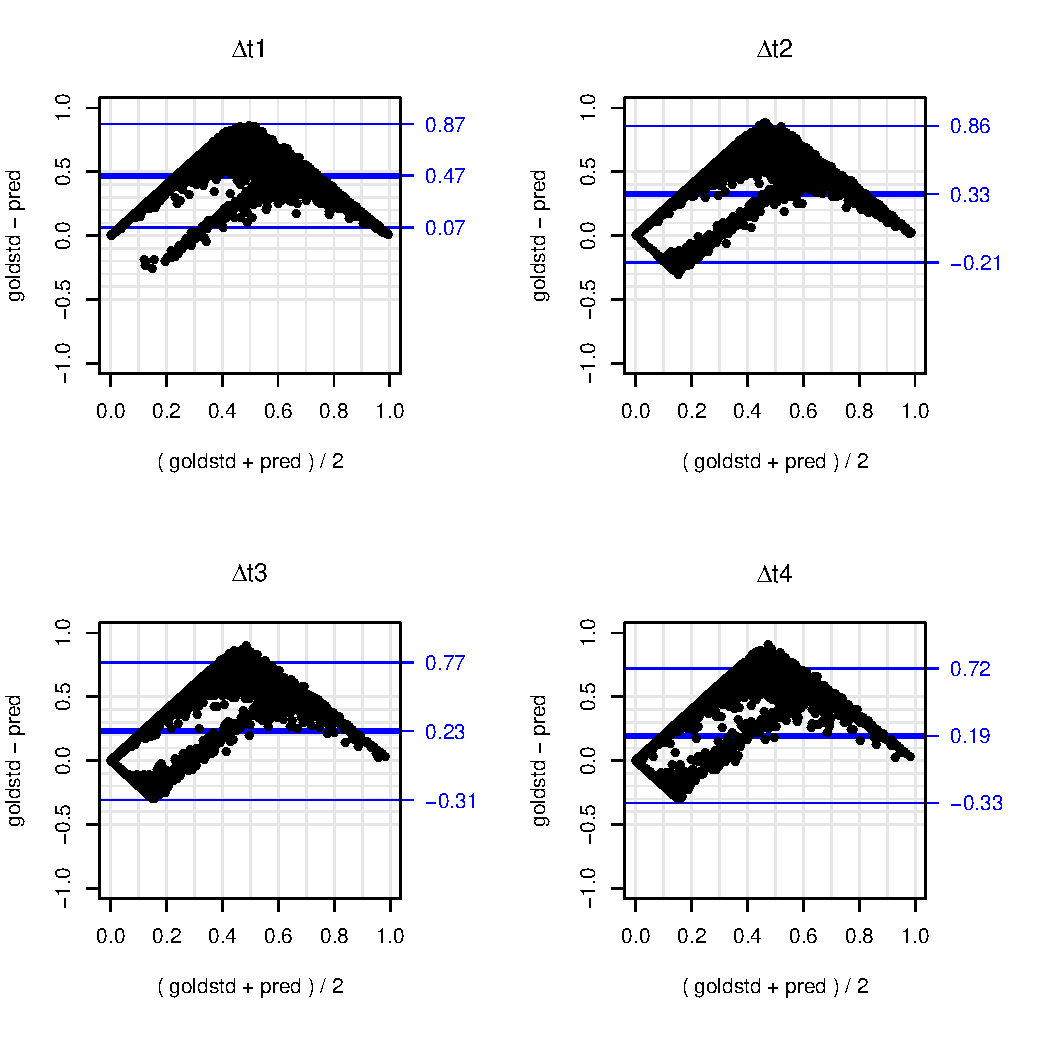
\includegraphics[width=0.45\columnwidth]{baplot_qt25data_LMJMfit_arms_t1.pdf}\label{plot:sim2fig13}
}
  \caption{Bland-Altman plot (bias and 95\% limits of agreement) of gold standard versus model predictions based on the first two longitudinal observations and four different prediction time intervals ($\Delta t_1 < \Delta t_2 < \Delta t_3 < \Delta t_4$) under Scenario 1.}
  \label{plot:sim2fig1}
\end{figure}

}


\frame{\frametitle{Simulation 2 results: Bland Altman plot (Cont'd)}
\begin{figure}[H]
\centering
\subfloat[][QRJM with $\tau=0.5$]{
    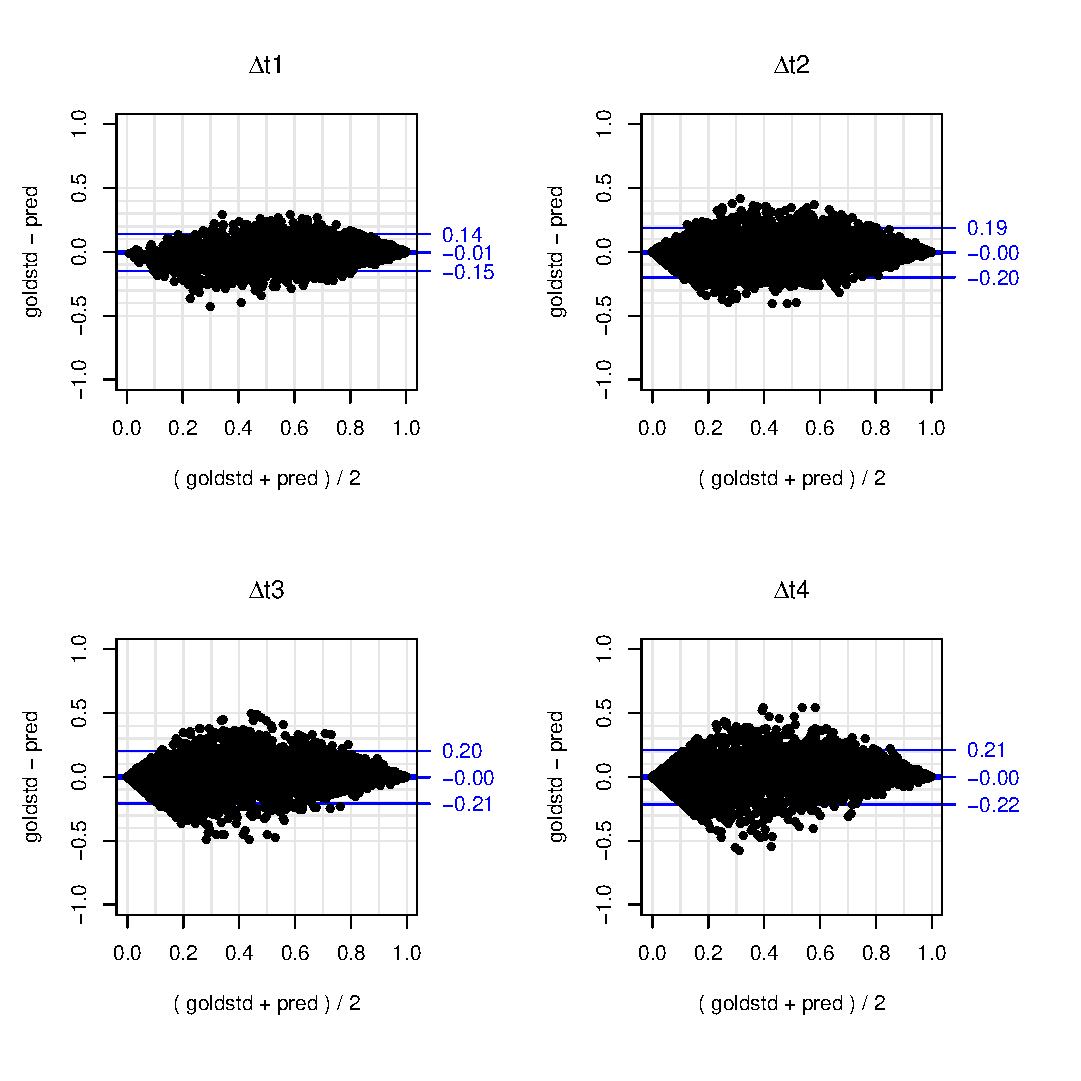
\includegraphics[width=0.45\columnwidth]{baplot_normdata_qt50fit_t1.eps}\label{plot:sim2fig31}
}
% \centering
% \subfloat[][QRJM with $\tau=0.5$]{
%     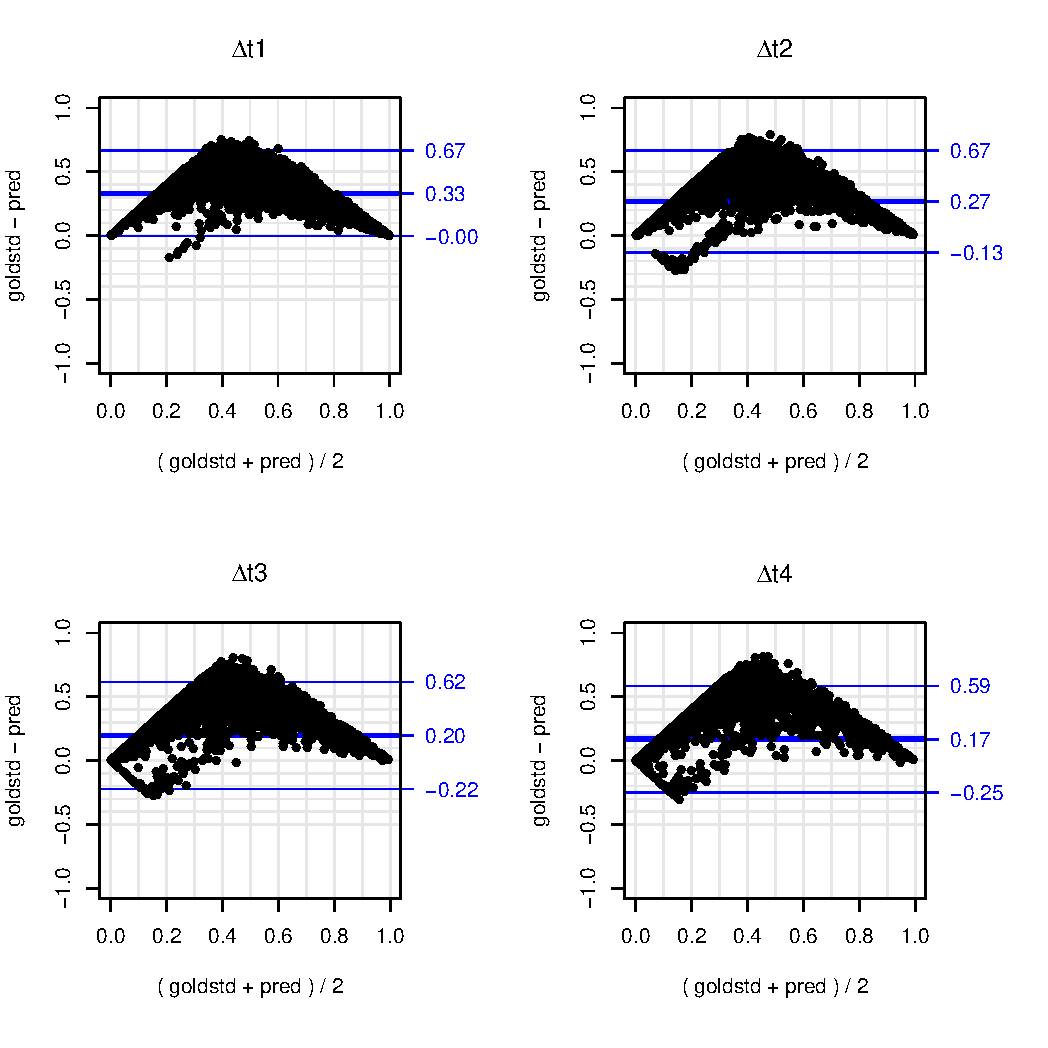
\includegraphics[width=0.4\columnwidth]{baplot_qt25data_qt50fit_jags_t1.pdf}\label{plot:sim2fig12}
% }
\subfloat[][LMJM (True model)]{
    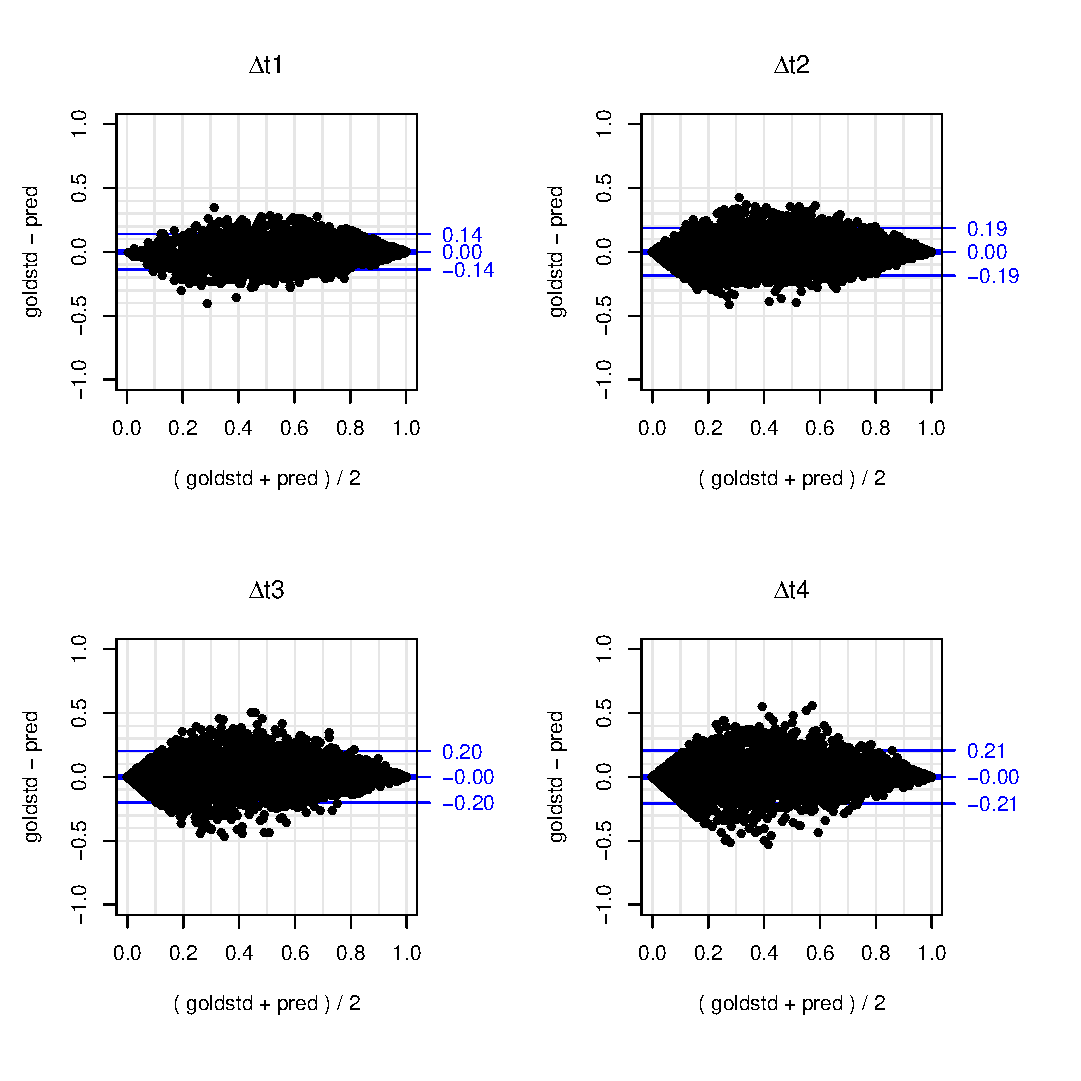
\includegraphics[width=0.45\columnwidth]{baplot_normdata_LMJMfit_t1.eps}\label{plot:sim2fig32}
}
  \caption{Bland-Altman plot (bias and 95\% limits of agreement) of gold standard versus model predictions based on the first two longitudinal observations and four different prediction time intervals ($\Delta t_1 < \Delta t_2 < \Delta t_3 < \Delta t_4$) under Scenario 3.}
  \label{plot:sim2fig2}
\end{figure}

}

\frame{\frametitle{Simulation 2 results: summary table}
\begin{table}[H]
\centering
\caption{Simulation study: MSE and bias of the difference between predicted survival probability and the gold standard (Scenario 1).}
\adjustbox{max width=\textwidth}{
\label{tab:sim2tab1}
\begin{tabular}{clcccccccc}
\hline
 & & \multicolumn{2}{c}{QRJM ($\tau=0.25$)} & &\multicolumn{2}{c}{QRJM ($\tau=0.5$)} & &\multicolumn{2}{c}{LMJM} \\
\cline{3-4}\cline{6-7}\cline{9-10}
$t$ & $\Delta t$ & MSE & Bias & & MSE & Bias & & MSE & Bias \\
\hline
\multirow{2}{*}{{\bf 0.25}} & 0.25 & 0.006 & 0.009 && 0.137 & -0.330 & & 0.244 & -0.462 \\
&  1 & 0.010 & 0.007 && 0.111 & -0.267 & & 0.177 & -0.343 \\
\multirow{2}{*}{(subjects left: 48.1\%)} &  2 & 0.012 & 0.003 && 0.083 & -0.197 & & 0.126 &-0.249 \\
&  3 & 0.013 & 0.000 && 0.072 & -0.168 & & 0.107 & -0.210 \\
\hline
\multirow{2}{*}{{\bf 0.5}} & 0.25 & 0.007 & 0.009 && 0.130 & -0.317 & & 0.219 & -0.439 \\
&   1 & 0.015 & 0.000 && 0.144 & -0.321 & & 0.221 & -0.408 \\
\multirow{2}{*}{(subjects left: 34.6\%)}&   2 & 0.017 & -0.015 && 0.121 & -0.259 & & 0.174 & -0.319 \\
&   3 & 0.018 & -0.023 && 0.109 & -0.228 & & 0.153 & -0.278\\
\hline
\multirow{2}{*}{{\bf 0.75}} & 0.25 & 0.009 & 0.005 && 0.125 & -0.301 & & 0.189 & -0.401 \\
& 1 & 0.023 & -0.007 && 0.174 & -0.356 & & 0.253 & -0.447 \\
\multirow{2}{*}{(subjects left: 22.8\%)} & 2 & 0.025 & -0.033 && 0.159 & -0.310 & & 0.218 & -0.375 \\
&  3 & 0.027 & -0.046 && 0.148 & -0.282 & & 0.197 & -0.336\\
\hline
\end{tabular}
}
\end{table}

}

%%%%%%%%%%%%%%%%%==DATA==%%%%%%%%%%%%%%%%%%%%%%%%
\section{Data application} %%%%%%%
\subsection{Data and model}
\frame{\frametitle{Data application}

\begin{itemize}
\item Split the 1078 study participants into two parts: a first sub-cohort of 800 participants is used to draw statistical inference for the unknown parameters; the remainder is used as test data for predictions of HD-free probability.


\item We consider the following joint models for our data analysis:
\begin{equation*}\label{eqn:data_joint}
\small{
\left\{
\begin{array}{l}
y_{i}(t) = m_{i}(t) + \varepsilon_{it} = \beta_0 + \beta_1 t+ \beta_2 age_{0i} + {u}_{i1} + u_{i2} t + \varepsilon_{i}(t),  \varepsilon_{i}(t)\sim ALD(0, \sigma, \tau)\\
h(T_i|\mathcal{M}_{i}(T_i);  \boldsymbol{\gamma}, \alpha) = \sum_{k=1}^3\lambda_kI_k(T_i)\exp(\gamma_1 education_i + \gamma_2 I_{male_i} + \alpha m_i(T_i))
\end{array}
\right.}
\end{equation*}
\item $y_{i}(t)$ represents one of the longitudinal biomarkers
\item $age_0$ is the baseline age at the enrollment.
\item Specify a piecewise constant baseline hazard function with three time intervals, where $\lambda_k$ is the hazard rate for time interval $[t_k, t_{k+1})$ and $I_k(t)=1$ if $t\in[t_k, t_{k+1})$ and 0 otherwise.
\end{itemize}
}


\subsection{Results}
\frame{\frametitle{Results}
\begin{table}[H]
\centering
\caption{PREDICT-HD data analysis: Parameter estimation and 95\% credible interval from QRJM at three different quantiles with TMS as the longitudinal biomarker.}
\label{realdata_inference}
\adjustbox{max width=\textwidth}{
\begin{tabular}{l ccc }
  \hline
  & \multicolumn{3}{c}{{total motor score}}\\
  \hline
  & $\tau=0.25$ & $\tau=0.50$ & $\tau=0.75$ \\
\hline
\multicolumn{2}{l}{\textit{longitudinal process}} & &\\
int. & -0.760 (-0.903, -0.628)& -0.525 (-0.699, -0.359)& -0.249 (-0.469, -0.035)\\

time (month) & 0.019 (0.015, 0.023)& 0.020 (0.016, 0.024)& 0.022 (0.018, 0.026)\\
$age_0$ & 0.004 (0.001, 0.008)& 0.005 (0.001, 0.010)& 0.006 (0.001, 0.012)\\

\multicolumn{2}{l}{\textit{time-to-event process}} & &\\
assoct. & 1.526 (1.321, 1.745)& 1.300 (1.148, 1.459)& 1.080 (0.968, 1.192)\\

eduyr & -0.083 (-0.115, -0.052)& -0.112 (-0.142, -0.082)& -0.128 (-0.157, -0.101)\\

male& 0.317 (-0.037, 0.654)& 0.360 (-0.020, 0.708)& 0.317 (-0.010, 0.647)\\
  \hline
\end{tabular}
}
\end{table}
}


\frame{\frametitle{Results (Cont'd)}
\begin{table}[H]
\centering
\caption{PREDICT-HD data analysis: AUC, AARD and MRD of the predictions of HD-free probability from QRJM and AUC from LMJM with TMS as the longitudinal biomarker.}
\label{tab:data_auc}
\adjustbox{max width=\textwidth}{
\begin{tabular}{rrrrrrrrrrrrrrc}
\hline
$t$ & $\Delta t$ & \multicolumn{3}{c}{AUC ($\tau$)} & & \multicolumn{3}{c}{AARD ($\tau$)} & & \multicolumn{3}{c}{MRD ($\tau$)} & & \multirow{2}{*}{AUC(LMJM)}\\
\cline{3-5}  \cline{7-9} \cline{11-13}
\multicolumn{2}{c}{(month)}  & 0.25 & 0.50 & 0.75 &  & 0.25 & 0.50 & 0.75&  & 0.25 & 0.50 & 0.75 & & \\
\hline
\multirow{3}{*}{$12$}  & 12 & 0.647 & 0.683 & 0.738 && 0.213 & 0.261 & 0.356 &&  0.010 & 0.020 & 0.059 & &0.679\\
            & 24 &  0.668 & 0.702 & 0.753 &&  0.244 & 0.290 & 0.379 && 0.028 & 0.054 & 0.128 && 0.695\\
            & 36 &  0.685 & 0.714 & 0.760 &&  0.273 & 0.311 & 0.391 && 0.054 & 0.091 & 0.170  & &0.693\\[0.5em]
\multirow{3}{*}{$24$}  & 12 & 0.836 & 0.857 & 0.864  && 0.539 & 0.575 & 0.577 &&  0.168 & 0.218 & 0.285 & &0.855\\
            & 24 &  0.852 & 0.872 & 0.873 && 0.566 & 0.598 & 0.583 && 0.285 & 0.361 & 0.404 & &0.878\\
            & 36 & 0.866 & 0.877 & 0.872 &&  0.581 & 0.599 & 0.575 && 0.368 & 0.420 & 0.430 & &0.836\\[0.5em]
\multirow{3}{*}{$48$}  & 12 &  0.875 & 0.878 & 0.868 &&  0.583 & 0.598 & 0.589 && 0.326 & 0.320 & 0.303 & &0.669\\
            & 24 & 0.875 & 0.883 & 0.874 && 0.578 & 0.602 & 0.598  &&  0.390 & 0.401 & 0.379 & &0.769\\
            & 36 &  0.877 & 0.887 & 0.879 && 0.589 & 0.614 & 0.599  && 0.417 & 0.439 & 0.417 & &0.774\\
\hline
\end{tabular}
}
\end{table}
}



\section{Discussion \& Conclusion}
\frame{\frametitle{Discussion \& Conclusion}
\begin{itemize}
\item The proposed JM provides a way to explore the covariates effect across the whole distribution span of the outcome variable. This becomes especially important when either the lower or higher quantile of the outcome becomes more relevant to the clinical interest.

\item Our proposed algorithm performs well in recovering the truth in inference and in making predictions of future survival probabilities.

% \item LMJM tended to provide biased point estimates as well as lower coverage probabilities for model parameters when the longitudinal data are skewed.

\item The best predictive performance from our model outperforms that from the LMJM when data are highly skewed.


\item Our novel application of JM in making personalized dynamic predictions of survival probability finds practical importance in many clinical applications.

\item Predictive accuracy criteria and/or other model selection methods or method(s), e.g. Bayesian model averaging, to incorporate multiple regression results from different quantiles into a single prediction solution can be helpful in selecting the ``best'' quantile in prediction.

\end{itemize}


}




%%%%%%%%%%%%%%%%%==Acknowledgement==%%%%%%%%%%%%%%%%%%%%%%%%
\section{Acknowledgement} %%%%%%%
\frame{\frametitle{Acknowledgement}
Sheng Luo Ph.D. and Stacia DeSantis Ph.D. are co-advisers of Ming Yang's dissertation work at UTSPH.  \\

\vspace{2em}
We would like to acknowledge the Texas Advanced Computing Center (TACC) for providing high-performing computing resources.

}




%%%%%%%%%%%%%%%%%==References==%%%%%%%%%%%%%%%%%%%%%%%%
 \section{References} %%%%%%%
\frame{\frametitle{Selected references}

\begin{thebibliography}{4}


 \beamertemplatearticlebibitems
  \bibitem{bland1986statistical}
    Bland, J. M. and Altman, D. G.
   \newblock Statistical methods for assessing agreement between two methods of clinical measurement.
    \newblock {\em The Lancet}, 327(8476):307--310, 1986.

 \beamertemplatearticlebibitems
  \bibitem{paulsen2014prediction}
    Paulsen, J. S., Long, J. D., Ross, C. A., Harrington, D. L., Erwin, C. J., Williams, J. K., Westervelt, H. J., Johnson, H. J., Aylward, E. H., Zhang, Y., et al.
    \newblock Prediction of manifest Huntington's disease with clinical and imaging measures: a prospective observational study.
    \newblock {\em The Lancet Neurology}, 13:1193--1201, 2014.


 \beamertemplatearticlebibitems
  \bibitem{kotz2001laplace}
    Kotz, S., Kozubowski, T., and Podgorski, K.
    \newblock The Laplace Distribution and Generalizations: A Revisit With Applications to Communications, Exonomics, Engineering, and Finance.
    \newblock {\em Springer}, 2001.

%  \beamertemplatearticlebibitems
%  \bibitem{guo2004separate}
%    Xu Guo and Bradley P Carlin
%    \newblock Separate and joint models of longitudinal and event time data using standard computer packages
%    \newblock {\em The American Statistician}, 58(1):16--24, 2004.
%


  \end{thebibliography}
}





\frame{\frametitle{Selected references (Cont'd)}
\begin{thebibliography}{4}

%  \beamertemplatearticlebibitems
%  \bibitem{brown2005flexible}
%    Elizabeth R Brown, Joseph G Ibrahim and Victor DeGruttola
%    \newblock A Flexible B-Spline Model for Multiple Longitudinal Biomarkers and Survival.
%    \newblock {\em Biometrics}, 61(1):64--73, 2005.


  \beamertemplatebookbibitems
  \bibitem{koenker2005quantile}
    Koenker, R.
    \newblock Quantile regression.
    \newblock {\em Cambridge university press}, 2005.

  \beamertemplatearticlebibitems
  \bibitem{Alessio2014qrjm}
    Farcomeni, A. and Viviani, S.
    \newblock Longitudinal quantile regression in the presence of informative dropout through longitudinal--survival joint models.
    \newblock {\em Statistics in Medicine}, 2015.

  \beamertemplatearticlebibitems
  \bibitem{rizopoulos2011dynamic}
    Rizopoulos, D.
    \newblock Dynamic Predictions and Prospective Accuracy in Joint Modelss for Longitudinal and Time-to-Event Data.
    \newblock {\em Biometrics}, 67(3):819--829, 2011.


  \beamertemplatearticlebibitems
  \bibitem{taylor2013real}
   Taylor, J. M., Park, Y., Ankerst, D. P., Proust-Lima, C., Williams, S., Kestin, L., Bae, K., Pickles, T., and Sandler, H.
    \newblock Real-time individual predictions of prostate cancer recurrence using joint modelss.
    \newblock {\em Biometrics}, 69(1):206--213, 2013.


  \end{thebibliography}


}

\frame{
  \centering
  {\bf \Large Thank you!}\\
  \vspace{2em}
  {\bf Questions?}
}




\end{document}